\subsubsection{20.01.15}
\begin{enumerate}
	
	\item Время начала и окончания собрания: 16:20 - 20:40.
	
	\item Цели собрания: 
	\begin{enumerate}
		
		\item Написать программу автономного периода при старте из зоны парковки.
		
		\item Продолжить тренировки.
		
	\end{enumerate}

	\item Проделанная работа:
	\begin{enumerate}
		
		\item Сегодня мы отладили программу автономного периода при старте с пандуса и, после этого, приступили к тренировкам. У нас уже стало лучше получаться. У нас получилось дважды набрать в ковш пять мячей и выкинуть их за 70 секунд. Наша задача научиться делать это трижды за 60 секунд.
		
		\item В процессе тренировки мы выяснили, что для захвата мячей достаточно двух лопастей, а 3-я только мешает захватывать их. 3-я лопатка была демонтирована.
        \begin{figure}[H]
	  	  \begin{minipage}[h]{0.2\linewidth}
	  	    \center  
	  	  \end{minipage}
	  	  \begin{minipage}[h]{0.6\linewidth}
	  		\center{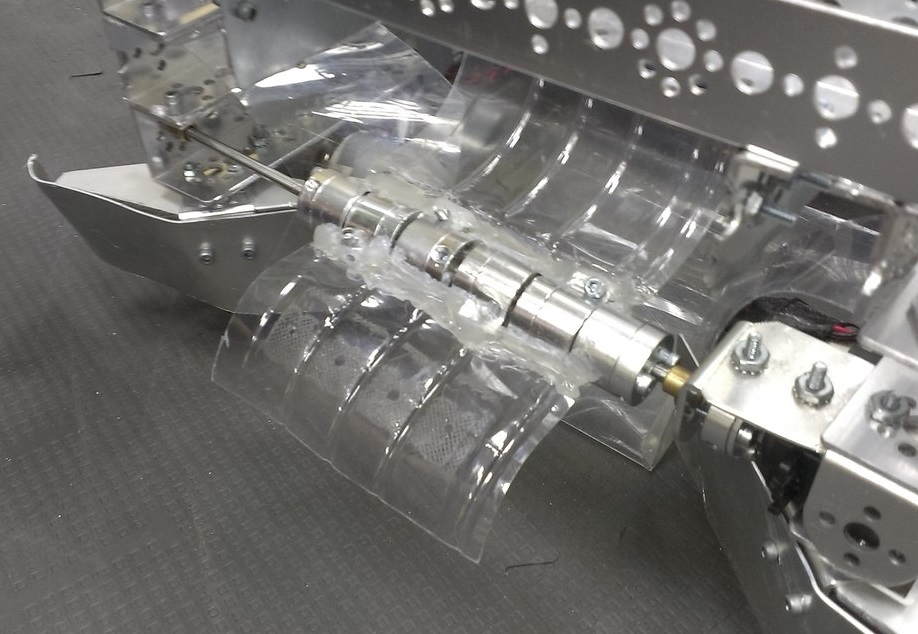
\includegraphics[scale=0.3]{days/20.01.15/images/01}}
	  		\caption{Захват мячей с 2-мя лопатками}
	  	  \end{minipage}
	   \end{figure}

	\end{enumerate}
	
	\item Итоги собрания:
	\begin{enumerate}
		
		\item Программа автономного периода при старте из зоны парковки не реализована.
		
		\item Программа автонома при старте с пандуса доработана.
		
        \item Тренировки прошли с пользой для операторов.
        
        \item Захват мячей был улучшен.
		
	\end{enumerate}
	
	\item Задачи для последующих собраний:
	\begin{enumerate}
		
		\item Продолжить тренировки.
		
        \item Написать программу автономного периода при старте из зоны парковки.
        	
	\end{enumerate}
\end{enumerate}
\fillpage
